\documentclass[letterpaper,12pt,oneside]{book}
%\usepackage[a4paper,includeall,bindingoffset=0cm,margin=2cm,marginparsep=0cm,marginparwidth=0cm]{geometry}
\usepackage[top=1in, left=0.9in, right=1.25in, bottom=1in]{geometry}
\usepackage{bachelorstitlepageUNAM}
\usepackage[utf8]{inputenc}
%%%%%%%%%%%%%%%%%%%%%%%%%%%%%
% Comparto una plantilla para la PORTADA que us\'e en mi t\'esis
% basada en el dise\~no gen\'erico que se usa en la Facultad de Ciencias
% Para usarlo \'unicamente aseg\'urate de tener la l\'inea
% \usepackage{bachelorstitlepageUNAM} y el archivo bachelorstitlepageUNAM.sty en el mismo directorio de trabajo.
% y los campos (sin signo %) :
%\author{Nombre del Alumno}
%\title{T\'itulo de la tesis}
%\faculty{Facultad}
%\degree{Grado que obtienes}
%\supervisor{ Tutor}
%\cityandyear{Ciudad y anio}
%\logouni{nombredelescudodelaunamsinespacios}
%\logofac{NombreDeLaImagenDelEscudodeTuFacultadSinEspacios}
% Para sugerencias y comentarios: DM en twitter.com/sglvgdor
% Subir\'e mas adelante la plantilla para maestr\'ia
%%%%%%%%%%%%%%%%%%%%%%%%%%%%%

%\author{Irving Yosafat Angel Camacho}
%\title{Métodos Numéricos de la Hidrodinámica Relativista aplicados a problemas de acreción y eyección en %jets astrofísicos}
%\faculty{Escuela Nacional de Estudios Superiores\\
%            Unidad Morelia}
%\degree{Licenciado en Geociencias}
%\supervisor{Dr. Sergio Mendoza Ramos \\ 
%Dr. Sinhué A. R. Haro Corzo}
%\cityandyear{Morelia, Michoacán, 2019}
%\logouni{Escudo-UNAM}
%\logofac{logo-enes}
%
%-------------------------------

%###################################
% Artículo 12.- El protocolo de tesis, con el visto bueno de un asesor, deberá ser entregado por 
% el alumno a la Coordinación de Carrera correspondiente para su registro, así como para su 
% presentación ante el Comité de Aprobación de Protocolo de Tesis correspondiente. El alumno 
% deberá tener un mínimo del 90% de créditos de su carrera para registrar su protocolo. La 
% Coordinación de Carrera será la responsable de realizar las gestiones académico-administrativas de 
% esta opción de titulación.
% Para someter el protocolo de tesis al Comité de Aprobación de Protocolo de Tesis respectivo, se 
% deberá entregar un documento que no exceda de cinco cuartillas, además de la portada, 
% considerando el contenido siguiente:
%    a) Portada, la cual deberá incluir: título del trabajo de tesis, nombre del alumno y nombre del asesor;
%    b) Objetivo(s) del trabajo;
%    c) Índice tentativo del trabajo de tesis;
%    d) Introducción, antecedentes y justificación del trabajo;
%    e) Metodología a emplear, y
%    f) Bibliografía básica (mínimo 10 referencias)
%###################################

\newcommand{\figura}[4]
{
  \begin{figure}[H]
    \centering
    \includegraphics[scale=#1]{#2}
    \caption{#3}
    \label{#4}
  \end{figure}
}
\newcommand{\refig}[1]{\figurename~\ref{#1}}
\newcommand{\reteo}[1]{$\mathfrak{Teorema}$~\ref{#1}}
\newcommand{\bb}[1]{\{#1\}}

%%Definiciones matemáticas
%\newtheorem{defi}{{\it Definici\’on}}[chapter]
\newtheorem{defi}{\textit{\textmd{$\mathfrak{Definición}$} }}
\newtheorem{teo}{\textit{\textmd{$\mathscr{TEOREMA}$} }}


%-----------------------__--------

\usepackage[T1]{fontenc}
\usepackage[utf8]{inputenc}
\usepackage[spanish,es-nodecimaldot,es-tabla]{babel}
\usepackage{graphicx}
\usepackage{tikz} 
\usepackage{tocloft}
\graphicspath{{./figs/}}
\usepackage{setspace}

%\usepackage[round]{natbib}

\renewcommand\cftsecpresnum{\S}
\renewcommand\cftsubsecpresnum{\S}   


\begin{document}
%------------------------------

    \begin{titlepage}
        \thispagestyle{empty}
        \begin{minipage}[c][0.17\textheight][c]{0.25\textwidth}
            \begin{center}
                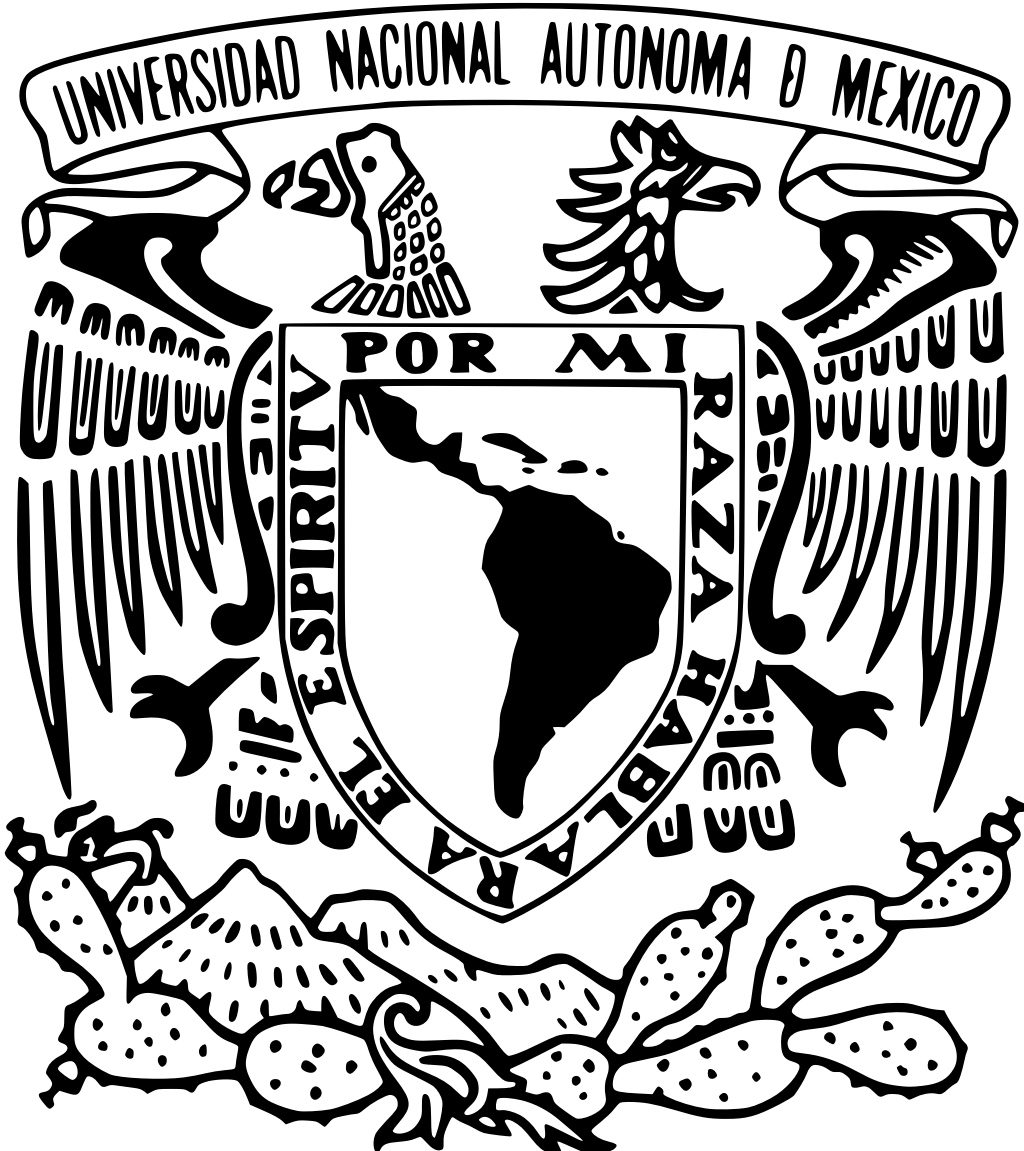
\includegraphics[width=3.5cm, height=3.5cm]{/home/aceron/Documentos/GitHub/Tesis/docTesis/Escudo-UNAM.png}
            \end{center}
        \end{minipage}
        \begin{minipage}[c][0.195\textheight][t]{0.75\textwidth}
            \begin{center}
                \vspace{0.3cm}
                \textsc{\large Universidad Nacional Aut\'onoma de M\'exico}\\[0.5cm]
                \vspace{0.3cm}
                \hrule height2.5pt
                \vspace{.2cm}
                \hrule height1pt
                \vspace{.8cm}
                \textsc{CENTRO DE FÍSICA APLICADA Y TECNOLOGÍA AVANZADA}\\[0.5cm] %
            \end{center}
        \end{minipage}

        \begin{minipage}[c][0.81\textheight][t]{0.25\textwidth}
            \vspace*{5mm}
            \begin{center}
                \hskip2.0mm
                \vrule width1pt height13cm 
                \vspace{5mm}
                \hskip2pt
                \vrule width2.5pt height13cm
                \hskip2mm
                \vrule width1pt height13cm \\
                \vspace{5mm}
                
\includegraphics[height=4.0cm]{/home/aceron/Documentos/GitHub/Tesis/docTesis/Esculo-CFATA.png}
            \end{center}
        \end{minipage}
        \begin{minipage}[c][0.81\textheight][t]{0.75\textwidth}
            \begin{center}
                \vspace{1cm}

                {\large\scshape Estudio de la precipitación pluvial en el estado de Querétaro usando datos del radar meteorológico ubicado en el Cerro de la Ronchera, Querétaro, en el periodo 2014-2019 para mostrar la viabilidad de los sistemas de almacenamiento de precipitación pluvial en la zona.}\\[.2in]

                \vspace{2cm}            

                \textsc{\LARGE T\hspace{1.5cm}E\hspace{1.5cm}S\hspace{1.5cm}I\hspace{1.5cm}S}\\[0.5cm]
                \textsc{\large que para obtener el t\'itulo de:}\\[0.5cm]
                \textsc{\large Licenciado en Tecnología}\\[0.5cm]
                \textsc{\large presenta:}\\[0.5cm]
                \textsc{\large {Ariel Cerón González}}\\[2cm]          

                \vspace{0.5cm}

                {\large\scshape Tutores:\\[0.3cm] {Dr. Adolfo Magaldi Hermosillo}}\\[.2in]

                \vspace{0.5cm}

                \large{Querétaro, Querétaro}{ }{2021}
            \end{center}
        \end{minipage}
    \end{titlepage}



%---------------------------------
\frontmatter
%\maketitle
% \chapter*{}
% \begin{flushright}%
%   \emph{Dedicatoria ...}
%   \thispagestyle{empty}
% \end{flushright}

% \chapter{Agradecimientos}
% \spacing{1.5}%\doublespacing

%\chapter{Notación}

\chapter{Introducción}
    En México, el manejo de los recursos hídircos es uno de los grandes temas de interes para diferentes sectores por el beneficio económico que genera. 
    Actualmente México enfrenta varias problemática sobre el recurso entre las que se encuentran el acceso al recurso para diferentes sectores de la población, la falta de lluvias originado por la tala inmoderada de bosques y selvas, sobre consesiones del recurso\cite{jornada:agua}, privilegios a clases sociales y falta de matenimiento a las instalaciones.

    Aunque en los últimos años se ha reconocido la importancia de cuidar y administrar el recurso \cite{de2019objetivo} \cite{mex:procaptar} son pocas las nuevas tecnologías o métodos que se han desarrollado para la solución del problema. 

    Una de las soluciones que más destaca es la de la captación del agua de lluvia \cite{comision2016lineamientos} \cite{hugues2019captacion} \cite{nickisch2018sistemas} \cite{van2013captacion} sin embargo las soluciones no consideran aspectos meteorológicos para su aplicación, sino que se realizan mediciones \textit{in situ} para validar la eficiencia del sistema.

    El aprovechamiento de tecnologías meteorológicas, como el radar, podrían dotar de más información que permita validar la eficiencia de sistemas, como el de capatación, sin la necesidad de realizar una instalación, ahorrando costos en la implementación del sistema o, por otro lado, eficientizandolos.

    \section{Hipótesis}
        Los registros históricos del radar meteorológico pueden proveer información sobre la densidad de precipitación pluvial y las zonas geográficas donde se condensa más este fenómeno. El correcto uso de los datos permitirá observar la evolución de la precipitación y la capacidad que tiene el estado para su aprovechamiento.

    \section{Objetivos}
        Conocer el comportamiento historio de la precipitación pluvial registrada con datos del radar meteorológico ubicado en el Cerro de la Ronchera para validar sistemas de recolección y almacenamiento de agua de lluvia.
        \subsection{Particulares}
            \begin{itemize}
                \item Generar mapas hídricos del estado de Querétaro para diferentes años y temporadas del año.
                \item Conocer y pronosticar la demanda hídirca del estado de Querétaro.
            \end{itemize}

    \section{Justificación}
        El estado de Querétaro ha presentado un crecimiento poblacional acelerado en los últimos años de su historio, lo que trae consigo mayor demanda de recursos básicos, entre los que destaca el acceso al agua. 
        El acceso al agua se ha visto comprometido de mayor forma en los últimos años y con ello la necesidad de contar con alternativas que permitan a la población contar con acceso al recurso. Uno de los métodos más populares es el de la cosecha de lluvia. Sin embargo la geografía del estado plantea una poblemática al momente de implementar esta solución.
        Al conocer las necesidades hídircas de la población, así como la capacidad puntual de precipitació facilitaría la implementación de tecnologías y políticas que permitan generar una mayor resilencia en el recurso.


\tableofcontents
%\listoffigures

    
\mainmatter

\chapter{Antecedentes} 
    El estado de Querétaro ha desarrollado problemas en relación con los recursos hídricos necesarios para satisfacer a la población, la industria y la agricultura. La disponibilidad del agua es la principal limitante del bienestar económico y social a largo plazo en la ciudad, pues el agua debe ser de una calidad acpetable, en cantidad adecuada y continua y a un precio razonable. Para confrontar las prioridades existentes relacionadas con el uso sosteneible de los recursos hídircos es necesario aprovechar todas las oportunidades existentes para la optimización de sus suministro, consumo y conservación.

    El hecho de que el abastecimiento del agua potable de la zona metropolitana de la ciudad de Querétaro (ZMCQ) provenga principalmente de un acuífero subterráneo sobreexplotado -Acuifero del Valle de Querétaro- representa un riesgo considerable para el gobierno y la sociedad, haciendo inevitable desarrollar estrategias y acciones específicas para garantizar el abasto de agua a largo plazo.

    Para lograr el abasto de agua es necesario generar la sustentabilidad\footnote{El desarrollo equitativo que cumple las necesidades del presente sin comprometer la habilidad de las generaciones futuras para cumplir sus propias necesidades} pasando por la conservación de sus fuentes, la lluvia, acuíferos, lagos, rios y bosques. Para el uso sustentable del agua se debe hacer una planeación completa fomentando el ahorro del recurso y aprovechar al máximo, sin sobreexplotar, las fuentes locales.

    Un método popular de aprovechamiento es el de la captación de agua de lluvia, llevando a desarrollar tesis \cite{comision2016lineamientos} \cite{hugues2019captacion} \cite{nickisch2018sistemas} \cite{van2013captacion} y guías técnicas para su instalación \cite{queralt2011agua} \cite{unatsabar2004guia}. En todas ellas se puede observar una base constante: un área de captación, un sistema de transporte y un lugar de almacenamiento. Variando uno a otro en técnologías extra como filtración, eliminación de bacterias, usuarios finales o materiales.

%Introudcción, antecedentes 

\chapter{El agua y su consumo}
    El problema de agua no es local ni se limita a una cierta región o país. El problema es global sin embargo, se presenta de forma más visible en cimunidades marginadas o paises menos desarrollados. Dentro de las causas más destacables se encuentra el crecimiento demográfico, la poca disponibilidad de agua dulce y su constante contaminación por actividades humanas.
    \section{El agua en Querétaro}
        \subsection{Tipos de consumidores}
        \subsection{Crisis}
    \section{Alternativas en el consumo}

\chapter{Precipitación Pluvial} 
    La atmósfera es un fluido complejo donde ocurren diferentes procesos. La suma de todos estos procesos es lo que conocemos coo tiempo atmosférico. Uno de los procesos que se desarrollan en la atmósfera es la precipitación pluvial, la cual se entiende como la caida del agua desde la atmósfera hacia la superficie terrestre.

    \section{Proceso de precipitación}
        El proceso de precipitación se puede relacionar con el ciclo del agua, sin embargo difiere de este al no considerar todas las etapas y enfocarse únicamente en la condensación y precipitación.
        \subsection{Nubes}
            Las nubes son cumulos inmesos de partículas \textit{suspendidas}\footnote{La velocidad en la caída de estas gotas es tan baja que parecen estar suspendidas} en la atmósfera, se forman cuando el aire se encuentra \textbf{saturado}. La saturación puede ocurrir por adición de gotas de agua, cristales de hielo, polvo o una mezcla de estos. 
            Cuando estas partículas se encuentran suspendidas en la atmosfera adquieren el nombre de \textbf{hidrometeoros}.
        \subsection{Precipitación}
            Los hidrometeoros se encuentran en constante movimiento en la atmosfera, generando colociones entre ellos que provocan el incremento en su tamaño. Los hidrometeoros tienen una variación en su tamaño que va desde los $2\mu m$ hasta los $2500 \mu m$. El aumento en el tamaño de los hidrometeoros genera un cambio en el peso de estos, haciendo que caigan hacia la superficie terrestre. Cuando esto le ocurre a una gran cantidad de hidrometeoros ocurre el fenómeno conocido como precipitación.
    \section{Métodos de medición}
        El volumen totoal de las precipitacciones que llegan a la superficie durante un período determinado se expresa en función del nivel que alcanzariían sobre una proyección horizontal de la superficie. La unidad de precipitación es la profundiad lineal, normalmente en milímetros. Los periódos comunies de observación son cada hora, cada tres horas y a diario, aunque en algunos casos se requiere una resolución temporal mucho mayor para medir intensidades de llvia muy elevadas.
        \subsection{Pluviómetros}
            Uno de los intrumentos de medición más utilizado es el pluviometro. El pluviometro es un recipiente abierto de lados vericales, en forma de cilindro recto, y con un embudo, cuya principal función es medir la lluvia puntual ocurrida en un periodo de tiempo determindado.
        \subsection{Medidores de precipitación registradores}
            Son aparatos que usan diferentes técnicas como el de pesaje, el cual registra el peso de la precipitación acumulada en un depósito, el de cubeta basculante, cuyo funcionamiento se basa en registrar el tiempo que tarda una cubeta en cambiar su inclinación esto en función de la precipitación ocurrida y el de flotador o pluviógrafo, en el cual la lluvia pasa a un recipiente que contiene un flotador y a medida qie el nivel del agua aumenta, el movimiento del flotador se transmite a un dispositivo que registra este cambio.

\chapter{Radar Meterorológico}
    El uso de radares en la meteorología tiene una gran historia desde su implementación, sin embargo el uso para aplicaciones hidrológicas es relativamente nuevo.
    \section{Funcionamiento}
        Un radar meteorológico es un emisor y receptor de pulsos electromagnéticos de duración $\tau$ y longitud de onda $\lambda$. 
        Cuando la energía emitida es interceptada por un \textit{blanco}, esta es dispersada en todas direcciones, de forma que una fracción de la energía es devuelta en dirección del radar y captada por el receptor. 
    \section{Aplicación en la meteorología}
        La medición de la energía electromagnética devuelta por una gota de lluvia está directamente relacionada con una cantdad física denomindad \textit{reflectivilidad} ($Z$) cuyas unidades son $mm^6/m^3$, a partir de esta unidad se puede conocer un estimado de la acumulación de la precipitación ($mm$) usando una relación conocida como $Z-R$ cuya ecuación esta dada en terminos de una ley de potencia del tipo $Z= aR^b$, con $a,b$ constantes determindas por factores como la ubicación y el tamaño de la gota. Usualmente se usan los parámtros empiricos de Marshall-Palmer tomando $a=200$ y $b=1.6$.

\chapter{Python}
    Python es un lenguaje de programación multiparadigma con estado OpenSource, lo cual ha promovido su uso de forma extensa en una basta cantidad de proyectos de todo tipo, entre los que destacan: desarrollo web, inteligencia artificial, estadística, modelos dinámicos  y aplicaciones de escritorio.
    Python es una excelente herramienta para el manejo y visualización de grandes cantidades de datos, además de que su aprendizaje es muy simple en compración de otros lenguajes existentes. 
    \section{Uso en la meteorología}
        Los radares meteorológicos usualmente empaquetan una gran cantidad de información como la ubicación, el tiempo en el que se muestreado, la cantidad de pulsos realizados, la inclinación del radar y todas y cada una de las mediciones. 
        Además de ello las diferentes empresas dedicadas a la fabricación de radares meteorológicos usan una codificación diferente para almacenar estos datos, haciendo que la utilización de los datos se vea afectada por no contar con los métodos de decoficiación necesarios. 
        Librerias de acceso público como \textbf{pyart} y \textbf{wradlib} facilitan este proceso al integrar diferentes algoritmos de decodificación para algunas marcas de radar, haciendo que su uso se vea limitado unicamente a las codificaciones que maneja.

\chapter{Metodología}
    \figura{1}{/home/aceron/Documentos/GitHub/Tesis/docTesis/metodo.png}{Diagrama de proceso}{fig:fig1}
    
%\chapter{Conclusiones}  
\nocite{*}
\bibliographystyle{apalike}
\bibliography{bibfile.bib}

\backmatter%@sglvgdor


\end{document}